\documentclass[14pt]{extarticle}


\usepackage[utf8]{inputenc}
\usepackage[russian]{babel}
\usepackage[top=3cm, bottom=2cm, left=2cm, right=1cm]{geometry}
\usepackage{indentfirst, pgfplots, float, amssymb, amsmath, caption, subcaption, listings}

\usepackage[hidelinks]{hyperref}

\linespread{1.25}

\captionsetup[figure]{labelsep=period}

\definecolor{mygreen}{rgb}{0,0.6,0}
\definecolor{mygray}{rgb}{0.5,0.5,0.5}
\definecolor{mymauve}{rgb}{0.58,0,0.82}
\definecolor{myblue}{rgb}{0.2,0,0.9}

\lstset{ %
  backgroundcolor=\color{white},    % choose the background color; you must add \usepackage{color} or \usepackage{xcolor}; should come as last argument
  basicstyle=\footnotesize\ttfamily,% the size of the fonts that are used for the code
  breakatwhitespace=false,          % sets if automatic breaks should only happen at whitespace
  belowcaptionskip=3em,
  breaklines=true,                  % sets automatic line breaking
  captionpos=b,                     % sets the caption-position to bottom
  commentstyle=\color{mygreen},     % comment style
  deletekeywords={...},             % if you want to delete keywords from the given language
  escapeinside={\%*}{*)},           % if you want to add LaTeX within your code
  extendedchars=true,               % lets you use non-ASCII characters; for 8-bits encodings only, does not work with UTF-8
  frame=single,	                    % adds a frame around the code
  keepspaces=true,                  % keeps spaces in text, useful for keeping indentation of code (possibly needs columns=flexible)
  keywordstyle=\color{myblue},      % keyword style
  language=C,                     % the language of the code
  morekeywords={uniform, out, layout, in, vec3, version, f32, s32, u32},
  numbers=left,                     % where to put the line-numbers; possible values are (none, left, right)
  numbersep=8pt,                    % how far the line-numbers are from the code
  numberstyle=\tiny\color{mygray},  % the style that is used for the line-numbers
  rulecolor=\color{black},          % if not set, the frame-color may be changed on line-breaks within not-black text (e.g. comments (green here))
  showspaces=false,                 % show spaces everywhere adding particular underscores; it overrides 'showstringspaces'
  showstringspaces=false,           % underline spaces within strings only
  showtabs=false,                   % show tabs within strings adding particular underscores
  stepnumber=1,                     % the step between two line-numbers. If it's 1, each line will be numbered
  stringstyle=\color{mymauve},      % string literal style
  tabsize=2,	                    % sets default tabsize to 2 spaces
  title=\lstname,                   % show the filename of files included with \lstinputlisting; also try caption instead of title
  belowskip=-2.0 \baselineskip,
  aboveskip=1.0 \baselineskip
}

\pgfplotsset{compat=1.17}

\begin{document}

%%%% Титульник %%%%
{
  \centering
  %	\includegraphics[scale=0.2]{logo.jpg}\\

  Федеральное государственное бюджетное образовательное\\ учреждение высшего образования\\
  \textbf{«Московский государственный университет\\ имени М. В. Ломоносова»}
  
  \noindent\rule{\textwidth}{1pt}
}

\noindent\begin{tabular}{@{}l l}
ФАКУЛЬТЕТ & Вычислительной математики и кибернетики\\
КАФЕДРА   & Cуперкомпьютеров и квантовой информатики 
\end{tabular}

\vfill

\begin{center}
  \centering
  \Large{\textbf{КУРСОВАЯ РАБОТА}}\\
  Сглаживание полигональных сеток методом Кэтмелла-Кларка
\end{center}

\vfill

\begin{flushright}
  \textbf{Студент}: Олохтонов Алексей Андреевич\\
  \textbf{Группа}: М-118\\
  \textbf{Научный руководитель}:
  Никольский Илья Михайлович\\
  к. ф.-м. н.
\end{flushright}

\begin{center}
  Москва, 2020
\end{center}

\thispagestyle{empty}
%%%% End of: Титульник %%%%

\newpage

\tableofcontents

\newpage

\section{Введение}
3D моделирование --- это трудоемкий и ресурсозатратный процесс, а потому попытки его упрощения предпринимаются уже очень давно. Для этой цели используются, например, неоднородные рациональные B-сплайны (NURBS), позволяющие 3D моделлеру задать набор контрольных параметров и получить гладкую поверхность, не моделируя ее самостоятельно \cite{rogers01}. Однако у NURBS есть и проблемы: возникают трудности с сшиванием двух соседних NURBS поверхностей, а также с созданием острых деталей, таких как сгибы и
углы. Также важной проблемой NURBS является то, что с их помощью нельзя представить поверхность произвольной топологии.

Эти и другие проблемы решает другой способ процедурного построения поверхностей: сглаживание за счет иерархического разбиения (surface subdivision). В таких алгоритмах вершины исходной полигональной сетки разными способами усредняются, и полученные новые вершины объединяются со старыми, образуя новую, более гладкую сетку.

Также важно отметить, что для комфортной работы 3D моделлера, реализация алгоритма должна позволять модифицировать модель в реальном времени, то есть весь процесс сглаживания должен занимать не более 16.7 мс.

Одним из самых популярных таких алгоритмов является метод Кэтмелла-Кларка, активно развиваемый студией Pixar Animation \cite{catmark79}. Изучению и реализации этого алгоритма и посвящена настоящая курсовая работа.

\begin{figure}[H]
    \centering
    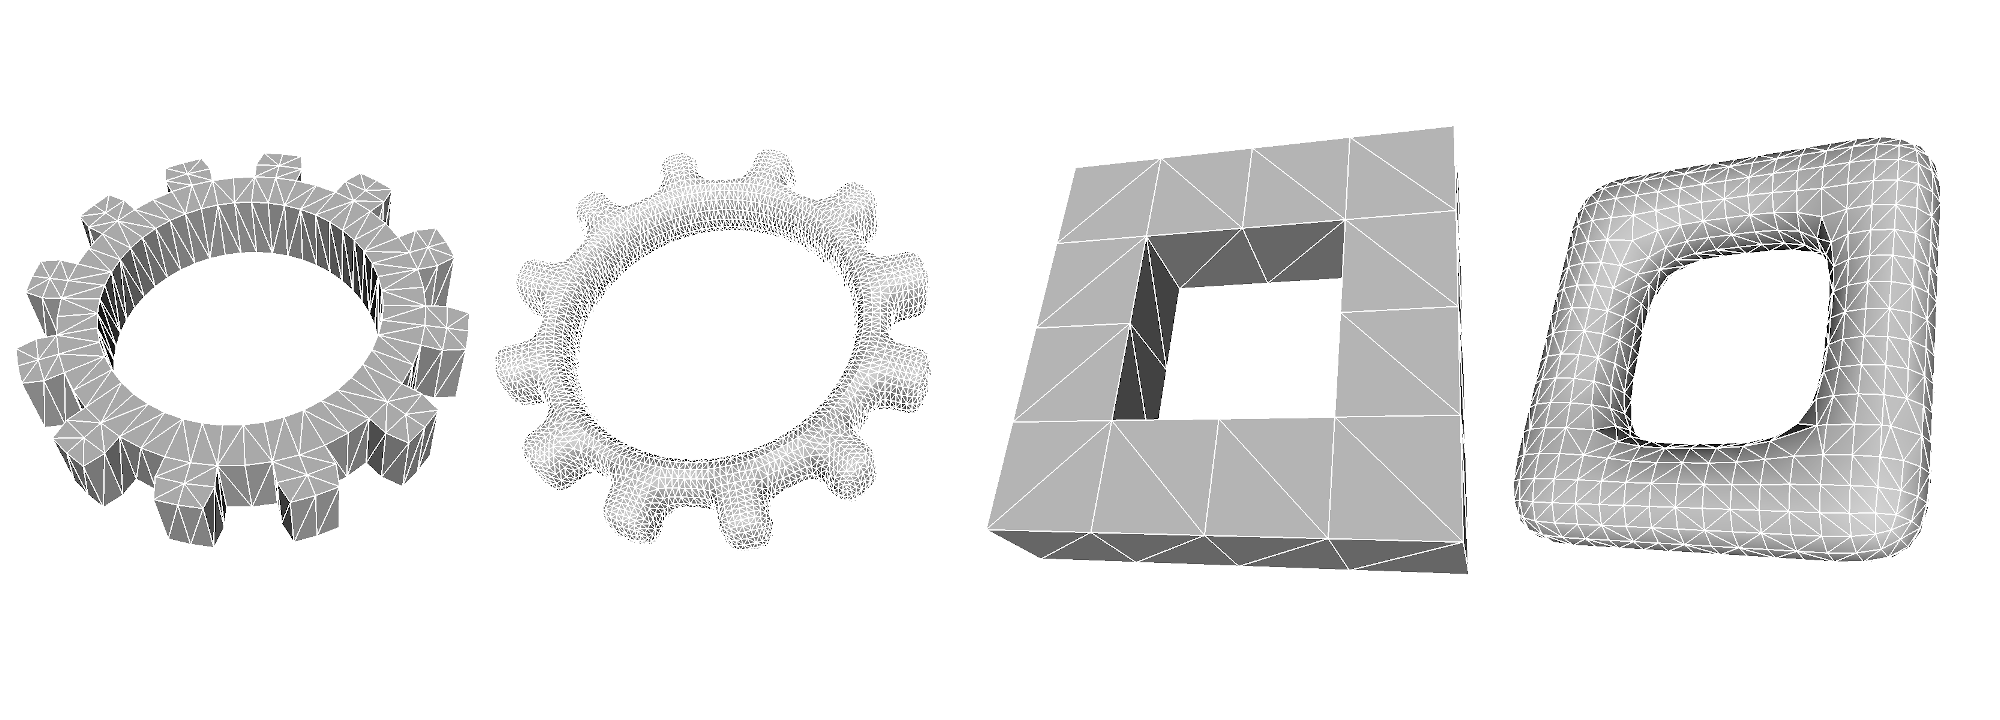
\includegraphics[scale=1.0]{gear_and_ct.png}
    \caption{Примеры оригинальных и сглаженных сеток}
\end{figure}

\newpage

\section{Постановка задачи}
Основной целью данной работы является изучение и реализация параллельного алгоритма Кэтмелла-Кларка для систем с общей памятью. В качестве целевой производительности принимается уровень, достигаемый в эталонной реализации OpenSubdiv от Pixar, а именно сглаживание сетки из 30,000 вершин на две итерации за временной бюджет реального времени \cite{opensubdivWWW}. Задачи, таким образом, включают:
\begin{enumerate}
    \item Ознакомление с алгоритмом Кэтмелла-Кларка и реализация рабочего прототипа программы
    \item Оптимизация последовательной версии программы
    \item Реализация параллельной версии программы (для систем с общем памятью), основанной на последовательной версии
\end{enumerate}

\newpage
\section{Метод Кэтмелла-Кларка}
Метод Кэтмелла-Кларка носит итерационный характер: исходная полигональная модель сглаживается, и полученная модель используется как входная для следующей итерации алгоритма. Итерации повторяются столько раз, сколько требуется для достижения необходимого уровня детализации. Каждую итерацию алгоритма можно условно разбить на два этапа: вычисление координат новых точек на основании старых, и построение граней из этих новых точек.

Отличие метода Кэтмелла-Кларка от других итерационных методов сглаживания заключается в том, как именно вычисляются новые точки, и как эти точки используются для построения новых граней. В методе Кэтмелла-Кларка существует три вида новых точек: первые называют \emph{точками граней (face points)}, вторые --- \emph{точками ребер (edge points)}, а третий тип точек не имеет собственного названия, и их расчет можно назвать \emph{пересчетом координат точек сетки}.

\subsection{Вычисление точек граней}
Координаты точек граней вычисляются как среднее арифметическое координат всех точек, составляющих данную грань. Другими словами, точка грани --- это барицентр соответствующей грани.

\begin{figure}[H]
  \centering
  \begin{tikzpicture}
    \begin{axis}[hide axis, ticks=none, xmin=-0.1, xmax=1.1, ymin=-0.1, ymax=1.3]
      \addplot3[patch, patch type=rectangle, color=yellow, fill opacity=0.5]
      coordinates {
        (0, 0, 0) (1, 0, 0) (1, 1, 0) (0, 1, 0.25)
      };
      \addplot3[mark=*]
      coordinates {
        (0, 0, 0) (1, 0, 0) (1, 1, 0) (0, 1, 0.25) (0, 0, 0)
      };
   %   \addplot3[mark=none, dashed]
%      coordinates {
 %       (0.5, 0.5, 0) (0.5, 0.5, 0.0625)
  %    };
      \addplot3[mark=*, black]
      coordinates {
        (0.5, 0.5, 0.0625)
      } node[above]{$F$};
    \end{axis}
  \end{tikzpicture}
  \caption{$F$ --- точка грани}
\end{figure}

Заметим, что точка грани не обязана лежать на этой грани.

\subsection{Вычисление точек ребер}
Назовем ребро смежным с гранью, если оно принадлежит к этой грани. В полигональных сетках у ребра чаще всего две смежных грани: так случается, когда полигональная сетка задает поверхность. Однако, ребро может быть смежно и одной грани, если оно находится на краю разреза.

\begin{figure}[H]
  \centering
  \begin{tikzpicture}
    \begin{axis}[hide axis, ticks=none, xmin=-0.1, xmax=1.1, ymin=-0.1, ymax=1.3]
      \addplot3[patch, patch type=rectangle, color=yellow, fill opacity=0.5, faceted color=black] coordinates { (0, 0, 0) (1, 0, 0) (1, 1, 0) (0, 1, 0.25) };
      \addplot3[patch, patch type=rectangle, color=orange, fill opacity=0.5, faceted color=black] coordinates { (1, 1, 0) (0, 1, 0.25) (0, 1.2, 0.5) (1, 1.2, 0.5) };
      \addplot3[color=black, line width=1.5pt] coordinates { (1, 1, 0) (0, 1, 0.25) };
      \addplot3[color=black, line width=1.5pt] coordinates { (1, 1, 0) (1, 0, 0) };
      \addplot3[mark=*, black] coordinates { (0, 1, 0.25) } node[left]{$A$};
      \addplot3[mark=*, black] coordinates { (1, 1, 0) } node[right]{$B$};
      \addplot3[mark=*, black] coordinates { (1, 0, 0) } node[right]{$C$};
    \end{axis}
  \end{tikzpicture}
  \caption{Ребро $AB$ смежно двум граням, а ребро $BC$ --- одной}
\end{figure}

В случае, если ребро смежно двум граням, его точка ребра вычисляется как среднее арифметическое между серединой этого ребра и серединой отрезка, соединяющего точки граней, смежных с данным ребром.

\begin{figure}[H]
  %\captionsetup{justification=raggedright,singlelinecheck=off}
  \begin{subfigure}{0.5\textwidth}
    \centering
    \begin{tikzpicture}
      \begin{axis}[hide axis, ticks=none, xmin=-0.1, xmax=1.1, ymin=-0.1, ymax=1.3]
        \addplot3[patch, patch type=rectangle, color=yellow, fill opacity=0.5, faceted color=black] coordinates { (0, 0, 0) (1, 0, 0) (1, 1, 0) (0, 1, 0.25) };
        \addplot3[patch, patch type=rectangle, color=orange, fill opacity=0.5, faceted color=black] coordinates { (1, 1, 0) (0, 1, 0.25) (0, 1.2, 0.5) (1, 1.2, 0.5) };
        \addplot3[dashed, black] coordinates { (1, 1, 0) (0, 1, 0.25) };
        \addplot3[mark=*, black] coordinates { (0, 1, 0.25) } node[left]{$A$};
        \addplot3[mark=*, black] coordinates { (1, 1, 0) } node[right]{$B$};

        \addplot3[mark=o, black] coordinates { (0.25, 0.25, 0.0625) } node[right]{$F_1$};
        \addplot3[mark=o, black] coordinates { (0.25, 1.1, 0.3125) } node[right]{$F_2$};

        \addplot3[mark=x, black] coordinates { (0.5, 1, 0.125) } node[above]{$M_2$};
        \addplot3[mark=x, black] coordinates { (0.25, 0.675, 0.1875) } node[left]{$M_1$};
        
        \addplot3[dashed, black] coordinates { (0.25, 0.25, 0.0625) (0.25, 1.1, 0.3125) };
        \addplot3[dashed, black] coordinates { (0.5, 1, 0.125) (0.25, 0.675, 0.1875) };

        \addplot3[mark=*, black] coordinates { (0.375, 0.8375, 0.15625) } node[below]{$E$};
      \end{axis}
    \end{tikzpicture}
  \end{subfigure}
  \begin{subfigure}{0.5\textwidth}
    $F_1, F_2$ --- точки граней, смежных с $AB$ \\
    $M_1$ --- середина отрезка $F_1F_2$\\
    $M_2$ --- середина отрезка $AB$\\
    $E = \frac{M_1 + M_2}{2}$ --- точка ребра $AB$
  \end{subfigure}
  \caption{$E$ --- точка ребра $AB$} 
\end{figure}

В случае, если ребро находится на краю разреза, точка ребра вычисляется как середина этого ребра.\\

\subsection{Пересчет координат точек сетки}
На данном этапе каждая точка $V$ полигональной сетки пересчитывается по следующей формуле:  
\begin{equation}\label{eq:v1}
  V' = \frac{F + 2E + (n - 3)V}{n},
\end{equation}
где $F$ --- среднее арифметическое всех точек граней, к которым принадлежит данная вершина, $E$ --- среднее арифметическое \emph{середин} ребер, к которым принадлежит данная вершина, $n$ --- количество граней, к которым принадлежит данная вершина. 

Возможно, что вершина лежит на краю разреза. Выполнение этого условия можно проверить, посчитав число граней и ребер, к которым принадлежит данная вершина. Если числа отличаются --- вершина лежит на краю разреза. В таком случае точки граней не учитываются, а среднее арифметическое середин ребер считается только для ребер, также принадлежащих к разрезу. Итоговая формула принимает вид:
\begin{equation}\label{eq:v2}
  V' = \frac{E_c + V}{n_c},
\end{equation}
где $E_c$ --- среднее арифметическое середин ребер, содержащих данную вершину, также принадлежащих к разрезу, $n_c$ --- количество ребер, содержащих данную вершину, принадлежащих к разрезу, $V$ --- старая координата вершины.

\subsection{Построение граней сглаженной сетки}
На последнем этапе алгоритма новые грани строятся из рассчитанных на предыдущих этапах точек. Для простоты рассмотрим построение в случае четырехугольной грани. Введем следующие обозначения: $A$, $B$, $C$, $D$ --- вершины грани, $F$ --- точка грани, $E_{AB}$, $E_{BC}$, $E_{CD}$, $E_{DA}$ --- точки соответствующих ребер. Тогда будет построено четыре четырехугольных грани: $[A, E_{AB}, F, E_{DA}]$, $[B, E_{BC}, F, E_{AB}]$, $[C, E_{CD}, F, E_{BC}]$ и $[D, E_{DA}, F, E_{CD}]$.

\begin{figure}[H]
  \centering
    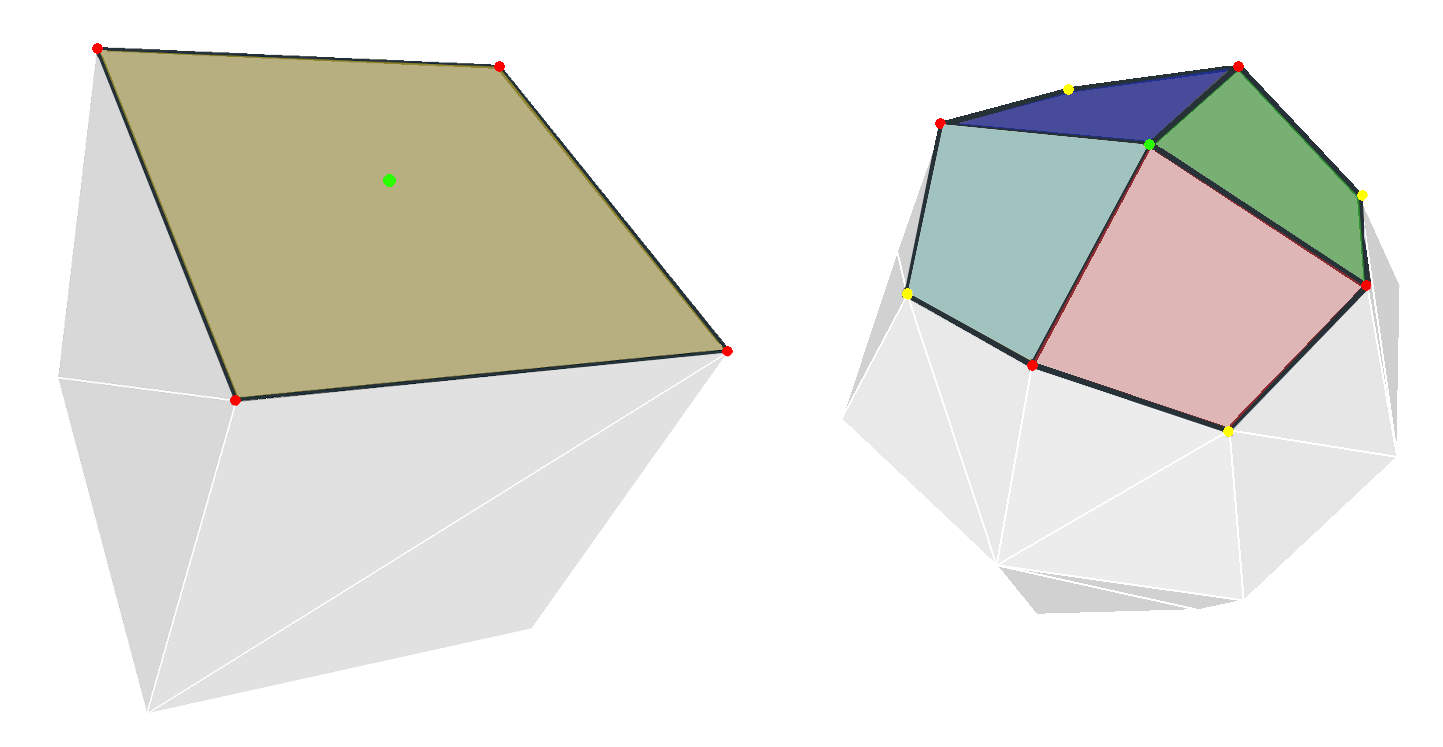
\includegraphics[scale=0.25]{subdiv.png}
    \caption{Разбиение четырехугольной грани}
\end{figure}

На рисунке исходная грань разбивается на четыре новых. Исходные вершины грани обозначены красным, точка грани --- зеленым, а точки ребер (отмечены только на втором рисунке) --- желтым. 

В общем случае имеем n вершин в разбиваемой грани и, соответственно, n точек граней. Новые грани строятся из следующих четырех вершин:
\begin{enumerate}
\item Вершина из сетки (заметим, что ее позиция пересчитана)
\item Точка ребра, соединяющего эту вершину со \emph{следующей} вершиной разбиваемой грани
\item Точка разбиваемой грани
\item Точка ребра, соединяющего эту вершину с \emph{предыдущей} вершиной разбиваемой грани
\end{enumerate}

\newpage
\section{Реализация последовательной программы}
Программа была реализована с использованием языка \texttt{C99}. В первую очередь была разработана последовательная версия программы, однако после реализации параллельной версии последовательная версия поддерживалась в актуальном состоянии, для того чтобы проводить честные сравнения производительности, так как параллельная программа, запущенная в один поток обычно медленнее последовательной. Для удобства переключение между одно- и многопоточной версией программы было реализовано через директиву препроцессора.

\subsection{Загрузка модели из файла во внутренний формат}
Прежде чем перейти к сглаживанию, необходимо загрузить модель с диска и преобразовать ее к некоторому внутреннему формату. Распространенными форматами хранения полигональным моделей на диске являются форматы \texttt{STL} и \texttt{Wavefront OBJ}. Для простоты был реализован только парсер формата \texttt{OBJ} \cite{objWWW}.

В формате \texttt{OBJ} полигональная сетка задается следующим образом: сначала перечисляются координаты вершин сетки, затем атрибуты этих вершин, такие как нормали и текстурные координаты, и наконец грани сетки, причем для обозначения вершины грани используются уже не координаты, а индекс вершины. Такой формат хранения позволяет избежать излишнего дублирования информации, которое неизбежно, к примеру, в формате \texttt{STL}. 

При разборе файла не учитывались никакие атрибуты вершин, кроме их позиции, и никакие атрибуты граней, кроме составляющих их вершин. Парсер был реализован в два прохода: первый проход подсчитывает количество вершин и граней, и под них выделяется память, а во втором проходе происходит непосредственно разбор вершин и граней, и они сохраняются в выделенной памяти.

Стоит заметить, что в более поздних версиях программы пришлось отказаться от использования библиотечных функций \texttt{strtod} и \texttt{strtof} в пользу самописных реализаций, так как для файлов размером более 100МБ больше времени уходило на разбор файла, чем на сглаживание, что сильно замедляло процесс тестирования и профилировки.

Внутреннее представление модели в программе практически совпадает с форматом \texttt{OBJ}: все координаты вершин сохраняются в отдельный массив, а грани представляют собой последовательность индексов. Также важно отметить, что ребра сетки в явном виде не хранятся. Вместо этого, ребра неявно заданы гранями: в последовательности индексов, задающих грань, ребро соединяет вершины, обозначенные подряд идущими индексами, а последняя вершина считается соединенной ребром с первой. Например, грань, содержащая индексы \texttt{1, 2, 3, 4}, неявно задает четыре ребра: \texttt{12, 23, 34, 41}. Также, для простоты индексации принимается, что все грани содержат одинаковое количество вершин.

\begin{lstlisting}[caption={Структура внутреннего представления сетки}, captionpos=b]
struct ms_v3 { f32 x; f32 y; f32 z; };
struct ms_mesh {
    struct ms_v3 *vertices;
    int *faces;
    int degree;
    int nverts, nfaces;
};
\end{lstlisting}

В выбранном представлении \texttt{vertices} --- массив длины \texttt{nverts}, а \texttt{faces} --- массив длины \texttt{nfaces * degree}, содержащий индексы, по которым в массиве \texttt{vertices} лежат координаты соответствующих вершин.

\subsection{Построение ускоряющей структуры}
Для вычисления точек ребер и пересчета координат точек сетки необходимо иметь доступ к информации о смежности: для точек ребер требуется знать к каким граням принадлежит данное ребро, а для пересчета координат необходим доступ ко всем смежным граням и смежным ребрам. Для организации эффективного доступа к этой информации была реализована ускоряющая структура.

Так как количество ребер, исходящих из данной вершины (как и количество граней, к которым эта вершина принадлежит) может быть разным для разных вершин, для каждой вершины необходимо иметь доступ к списку и длине этого списка.

Здесь нужно заметить, что каждая вершина однозначно представляется своим индексом, а индексы плотно упакованы (то есть для каждого индекса из промежутка \texttt{0...nverts - 1} есть вершина). А значит, списки можно хранить в виде разреженной матрицы в формате \texttt{CSR}.

Также заметим, что ребро однозначно определяется своим началом и концом, а потому вместо смежных ребер достаточно хранить смежные вершины. Тогда, некоторая точка \texttt{A} будет принадлежать всем ребрам, которые начинаются в вершине \texttt{A}, а заканчиваются в вершинах, смежных с \texttt{A}.

Смежные грани хранятся аналогично, во второй разреженной матрице.
\begin{lstlisting}[caption={Ускоряющая структура}, captionpos=b]
struct ms_accel {
    int *faces_starts; /* offsets for faces_matrix */
    int *verts_starts; /* offsets for verts_matrix */
    int *faces_matrix; /* adjacent faces CSR */
    int *verts_matrix; /* adjacent vertices CSR */
    int *edge_indices; /* edge_index[2 * e + 0], edge_index[2 * e + 1] */
};
\end{lstlisting}

Важно заметить, что как при вычислении точек ребер, так и при пересчете координат точек сетки, необходимо чтобы смежные точки и грани не дублировались. При пересчете координат это необходимо, так как вычисляется среднее арифметическое (середин ребер и точек граней). В вычислении точек ребер отсутствие дубликатов необходимо, так как гарантирует, что одни и те же точки граней не будут вычислены несколько раз и записаны в новую сетку как уникальные.

Таким образом, ускоряющая структура должна содержать для каждой вершины: список уникальных смежных вершин, и список уникальных смежных граней. Создание ускоряющей структуры было реализовано в три этапа:
\begin{enumerate}
\item Подсчет всех смежных вершин и граней (а не только уникальных). Этот этап необходим, чтобы рассчитать максимально возможные сдвиги в разреженной матрице, так как все данные записываются в один массив.
\item По рассчитанным сдвигам будут записываться смежные вершины и грани, причем вершина или грань не добавляются, если для данной вершины они уже добавлены.
\item Из полученного массива удаляются ``дырки'': так как сдвиги были рассчитаны в худшем случае, между концом одного списка и началом следущюего практически наверняка будет несколько пустых элементов. Эти интервалы заполняются за счет переупаковки массива. После упаковки становится ненужным хранить длины списков, так как они вычисляются вычитанием предыдущего сдвига из следующего, как это обычно делается в формате \texttt{CSR}. % тестирование - это плюс
\end{enumerate}

Наконец, заметим, что в полигональной сетке любое ребро встречается либо два (обычный случай), либо один (ребро находится на края разреза) раз. Это означает, что любому ребру можно поставить в соответствие два числа (в случае разреза эти числа будут равны), так что в совокупности все эти числа полностью заполнят промежуток \texttt{0...(nfaces * degree)}. Это необходимо, чтобы организовать быстрый доступ к точке данного ребра для данного ребра.

\begin{lstlisting}[caption={Добавление смежной вершины с проверкой уникальности}, captionpos=b]
int edge_base = edge_bases[start];
int edge_count = edge_counts[start];   
int found = -1;
  
for (int e = edge_base; e < edge_base + edge_count; ++e) {
    if (edges[e] == end) { found = e; break; }
}
  
if (found_1 == -1) {
    edge_counts[start] += 1;
    edges[edge_base + edge_count] = end;
    edge_indices[(edge_base + edge_count) * 2 + 0] = edge_index_1;
    edge_indices[(edge_base + edge_count) * 2 + 1] = edge_index_1;
} else {
    edge_indices[found * 2 + 1] = edge_index_1;
}
\end{lstlisting}

\subsection{Вычисление точек граней и точек ребер}
Точки граней вычисляются простым проходом по всем граням, в котором координаты вершин грани усредняются и записываются по индексу, соответствующему номеру грани.

Для расчета точек ребер итерация происходит не по граням, а по вершинам, которые принимаются за начало грани. Затем, для данной вершины происходит проход по всем уникальным концам ребер с началом в данной вершине. Полученные индексы используются для расчета середины ребра, а индексы смежных к ребру граней получаются делением индекса ребра на количество вершин в грани. Если смежные грани не равны, то происходит расчет по стандартной формуле,
% TODO вынести в формулу и сослаться
в противном же случае используется просто середина ребра. Полученная точка записывается по двум индексам, соответствующим данному ребру. Также, используется специальное значение \texttt{-1}, обозначающее что для данного ребра точка ребра еще не расчитана. Так как ребра могут встретиться в ускоряющей структуре два раза (один раз в списке вершин, смежных с началом ребра, и второй --- в списке вершин, смежных с концом ребра), то перед расчетом точки проверяется, что она еще не заполнена. В случае, если точка уже посчитана --- повторные расчеты не производятся.
\begin{lstlisting}[caption={Расчет и сохранение точек ребер}, captionpos=b]
for (int start = 0; start < mesh.nverts; ++start) {
    int from = accel.verts_starts[start];
    int to = accel.verts_starts[start + 1];        
    for (int e = from; e < to; ++e) {
        int eidx_1 = accel.edge_indices[2 * e + 0];
        int eidx_2 = accel.edge_indices[2 * e + 1];        
        if (edge_points[edge_index_1] != -1) { continue; }         
        /* compute edge point. face_1 = eidx_1 / mesh.degree, face_2 = eidx_2 / mesh.degree */
        ...
        edge_pointsv[nedge_pointsv] = edge_point;            
        edge_points[eidx_1] = nedge_pointsv;
        edge_points[eidx_2] = nedge_pointsv; 
        ++nedge_pointsv;
    }
}
\end{lstlisting}

Координаты всех уникальных точек ребер записываются в отдельный массив, который будет составлять часть массива координат сглаженной сетки.

\subsection{Пересчет координат точек сетки}
Для пересчета координат точек сетки происходит итерация по всем вершинам. Для каждой вершины из ускоряющей структуры читается количество смежных вершин и граней. Если эти значения равны, координата точки вычисляется по формуле \eqref{eq:v1}, иначе по формуле \eqref{eq:v2}.

Стоит заметить, что для проверки условия ``ребро также принадлежит разрезу'' происходит поиск в ускоряющей структуре индексов данного ребра, и эти индексы сравниваются: равные индексы означают, что ребро принадлежит только одной грани, то есть лежит на краю разреза. Неравные индексы означают, что ребро обыкновенное, и не должно учитываться при расчете.

Наконец, важно, что пересчитанные координаты точек сетки записываются в новый массив, а не переписываются поверх старых, потому что старые координаты вершины могут пригодиться для пересчета остальных точек.
\begin{lstlisting}[caption={Пересчет координат точек сетки}, captionpos=b]
for (int v = 0; v < mesh.nverts; ++v) {
    struct ms_v3 vertex = mesh.vertices[v];
    struct ms_v3 new_vert;
       
    int adj_verts_count = accel.verts_starts[v + 1] - accel.faces_starts[v];
    int adj_faces_count = accel.faces_starts[v + 1] - accel.faces_starts[v];
        
    if (adj_faces_count != adj_verts_count) {
        new_vert = ...;
    } else {
        new_vert = ...;
    }

    new_verts[v] = new_vert;
}
\end{lstlisting}


\subsection{Построение граней сглаженной сетки}
Построение новой, сглаженной сетки происходит в два этапа: копирование координат уникальных точек и создание новых граней.

Координаты новых точек собираются из трех массивов: координат точек сетки, точек ребер и точек граней.
\begin{lstlisting}[caption={Сборка нового массива координат}, captionpos=b]
memcpy(new_mesh.vertices, new_verts,
       mesh.nverts * sizeof(struct ms_v3));
memcpy(new_mesh.vertices + mesh.nverts, edge_pointsv,
       nedge_pointsv * sizeof(struct ms_v3));
memcpy(new_mesh.vertices + mesh.nverts + nedge_pointsv, face_points,
       mesh.nfaces * sizeof(struct ms_v3));
\end{lstlisting}

Построение новых граней происходит в соответствии с алгоритмом, за тем исключением, что вместо координат вершин используются их индексы в только что составленном массиве.

Сгенерированная сетка по формату соответствует сетке, полученной на вход, поэтому может быть повторно сглажена.

\newpage
\section{Реализация параллельной программы}
Для реализации параллельной версии программы были использованы средства \texttt{OpenMP}.

\subsection{Построение ускоряющей структуры}
Три основных этапа построения ускоряющей структуры: подсчет неуникальных ребер, поиск и устранение дубликатов, плотная упаковка, были распараллелены разными способами.

Для параллельного подсчета неуникальных ребер была заведена копия счетчиков на каждом потоке. Далее, прежде чем сливать все массивы счетчиков в один, происходило ``распространение'' сдвигов внутри каждого потока: на место каждого счетчика записывалась сумма всех предыдущих. Этот шаг производился в параллельной версии раньше, так как на уже слитом массиве его сложно распараллелить. Наконец, массивы сливались в один, причем каждый поток отвечал не за свой массив, а за свой диапазон индексов. Таким образом, была получна полностью параллельная реализация первого шага построения ускоряющей структуры.

Этап поиска и устранения дубликатов был распараллелен по модели \texttt{SPMD}, так как для избавления от блокировок и взаимных исключений необходимо гарантировать, что один и тот же список смежных вершин (или граней) всегда будет обрабатываться один и тем же потоком. Для этого все вершины были разбиты на равные промежутки, каждый из которых обрабатывался только один потоков. Однако из-за того, что порядок ребер имеет, вообще говоря, непредсказуемый характер, каждому потоку приходилось исполнять все итерации внешнего цикла, и на каждой итерации проверять условие попадания рассматриваемой вершины в промежуток. Если вершина попадает в промежуток, выделенный данному потоку, то она обрабатывалась, иначе --- пропускалась.

Распараллелить плотную упаковку матрицы, вообще говоря, не удалось. Однако, с помощью конструкции \texttt{omp sections} упаковки смежных вершин и граней были выделены в независимые задачи.

\subsection{Расчет новых точек и построение граней}
Природа вычисления точек граней и пересчета координат точек сетки позволила распараллелить их с использованием конструкции \texttt{omp for}. Аналогично был распараллелен этап построения граней сглаженной сетки: индексы для записи в массив граней однозначно определяются номером самой грани.

Вычисление точек ребер также не имеет зависимостей между итерациями, однако для того, чтобы исключить конфликты записи между потоками, итерации цикла были распределены по следующей схеме: каждый поток получал промежуток вершин (начал ребер) для обработки, а также отступ в массиве координат. Далее, поток обрабатывает только те ребра, начала которых попадают в выделенный промежуток, а координаты результирующих точек записывает с учетом полученного отступа.

\subsection{Параллелизм за счет независимости этапов}
Некоторые этапы работы алгоритма (особенно те, которые обрабатывают ребра), страдают от неравномерного распределения работы между потоками, потому что по выбранному диапазону вершин нельзя точно оценить, сколько ребер начинается в этих вершинах. Особенно хорошо это заметно на этапах удаления дубликатов при построении ускоряющей структуры и при вычислении точек ребер. На рисунках каждый поток обозначен цветным столбцом, пробелы между столбцами означают простой потоков.

\begin{figure}[h]
  \centering
    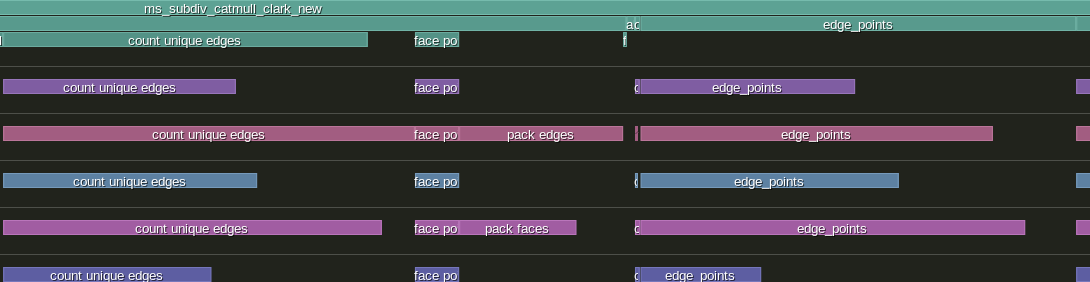
\includegraphics[scale=0.45]{bad_threads.png}
  \caption{Простой потоков из-за неравномерности нагрузки}
\end{figure}

Однако, построив граф зависимости по данным между этапами работы алгоритма, можно заметить, что некоторые этапы не зависят от результатов работы других \cite{voevodin02}. Так, вычисление точек граней не зависит от построения ускоряющей структуры, так как не использует ее. Поэтому, освободившиеся от устранения дубликатов потоки можно направить на вычисление точек граней. Аналогично, этап пересчета координат точек граней не использует точки ребер, а потому может быть начат потоком сразу же. Для реализации этих преобразований достаточно удалить из ключевых мест директиву \texttt{omp barrier}, и добавить идущим за ними циклам клаузу \texttt{schedule(guided)}.

\begin{figure}[H]
    \centering
    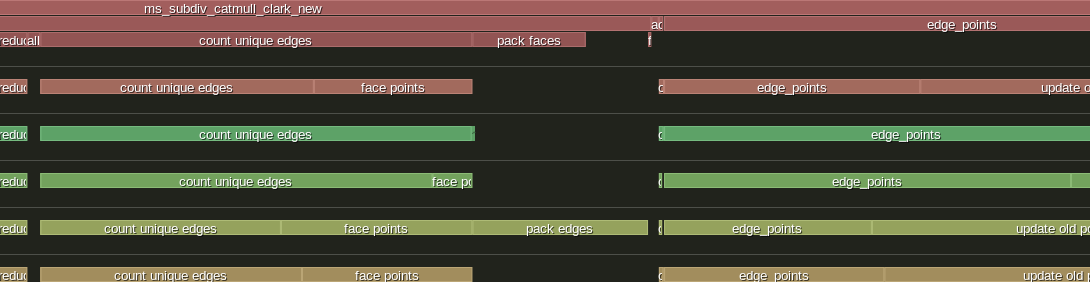
\includegraphics[scale=0.45]{good_threads.png}
    \caption{Простой потоков устранен за счет независимых задач}
\end{figure}

Аналогично можно совместить этапы последнего шага алгоритма: копирование координат уникальных точек и построение граней сглаженной сетки. Однако, профилировка показала, что этап построения новых граней ограничен пропускной способностью памяти, и добавление одновременного этапа копирования информации не ускоряет, а только замедляет программу.

\newpage
\section{Тестирование и профилировка}
Процесс тестирования был сосредоточен в основном на измерении производительности, однако на этапе разработки первого рабочего прототипа программы внимание уделялось именно корректности работы программы. 

Для простоты в программу не включалась никакая визуализация, вместо этого пользователю предлагается возможность сохранить полученную сетку в формате \texttt{OBJ} на диск. Для визуализации же пользователь может воспользоваться любой программой, способной отобразить файлы в этом формате.
%\begin{figure}[H]
%    \centering
%    \begin{subfigure}{0.45\textwidth}
%        \includegraphics[scale=0.22]{torus_0.png}
%    \end{subfigure}
%    \begin{subfigure}{0.45\textwidth}
%        \includegraphics[scale=0.22]{torus_6.png}
%    \end{subfigure}
%\end{figure}

\subsection{Инструментарий}
Для отображения \texttt{OBJ} моделей использовалась программа \texttt{view3dscene}. Замеры производительности внутри программы производились с помощью библиотечной функции \texttt{clock\_gettime} (для оценки времени работы в миллисекундах) и инструкции \texttt{rdtsc} (для оценки времени работы в процессорных циклах). Для профилировки использовался профилировщик \texttt{Tracy}, а также \texttt{AMD uProf} при запуске на процессоре \texttt{AMD} и \texttt{Intel VTune}
\cite{kasper03} при запуске на процессоре \texttt{Intel}.

Оценка времени работы внутри программы использовалась для вывода таких метрик, как ``количество процессорных циклов на вершину'' и ''время, затраченное на N шагов сглаживания``, которые использовались для сравнения общей производительности разных версий программы и для сравнения производительности с другими реализациями метода Кэтмелла-Кларка.

Профилировщики \texttt{Tracy} использовался для оценки распределения времени работы программы на уровне более гранулярном чем функции, а также для оценки эффективности работы потоков параллельной версии программы.

Профилировщики \texttt{AMD uProf} и \texttt{Intel VTune} использовались для оценки эффективности использования процессора на микроархитектурном уровне, а также для доступа к процессорным счетчикам, таким как количество кеш-промахов, неверных спекуляций и прочих.

\subsection{Корректность}
Для проверки корректности сглаживались специально созданные простые модели, корректность сглаживания которых легко проверить визуально: куб, который превращается в подобие сферы, куб с удаленной гранью, который превращается в подобие чаши.

\begin{figure}[H]
    \centering
    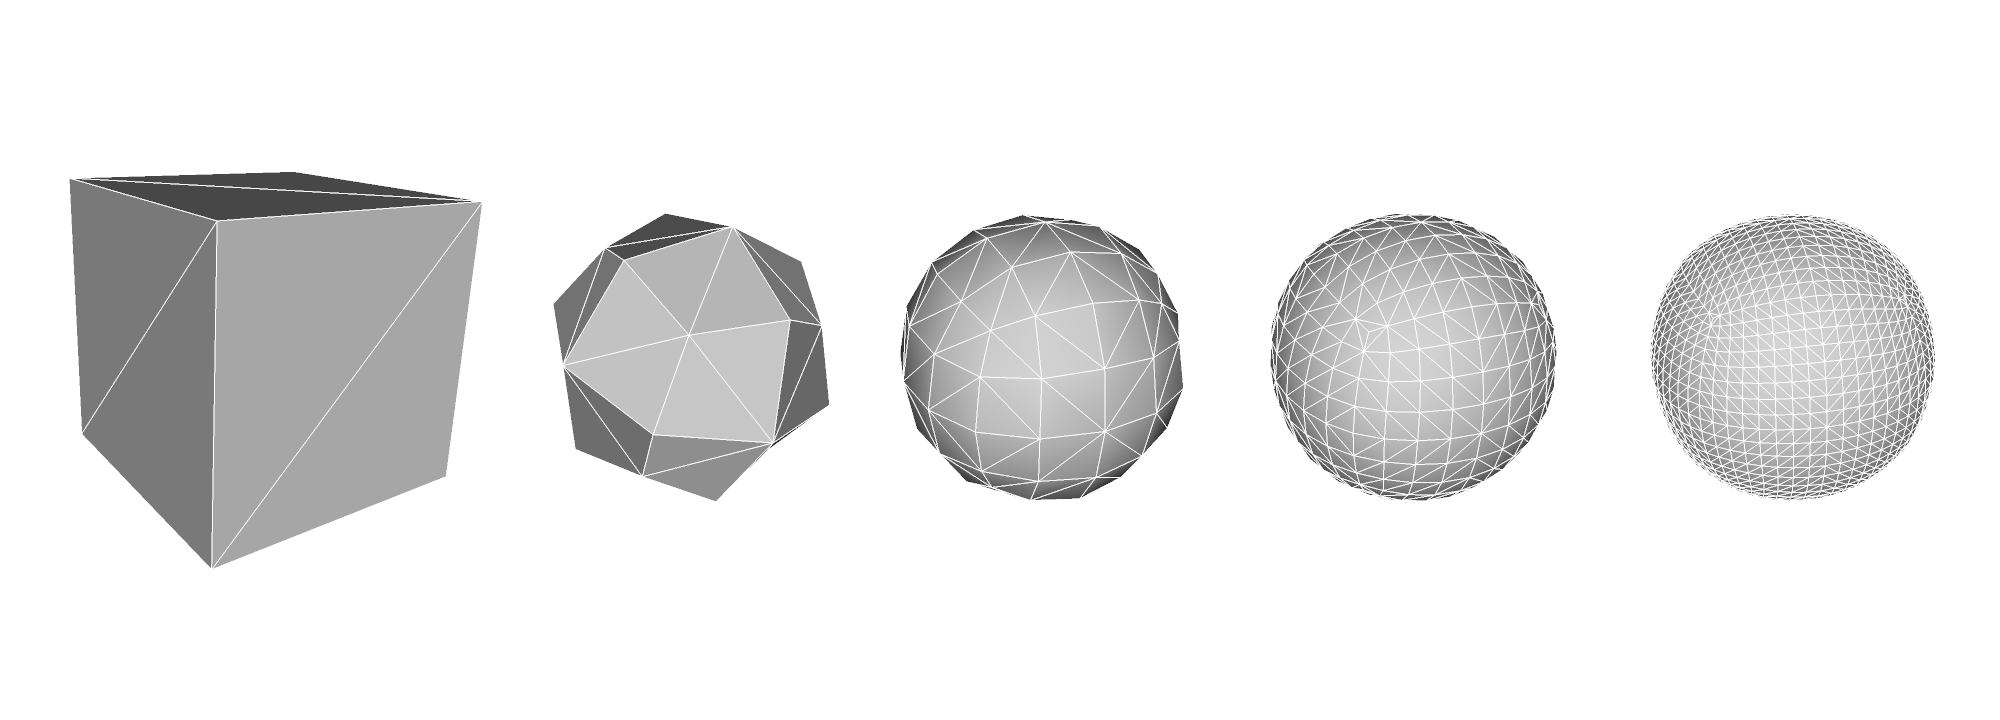
\includegraphics[scale=1.0]{cubes.png}
    \caption{Пять итераций сглаживания модели куба}
\end{figure}

\begin{figure}[H]
    \centering
    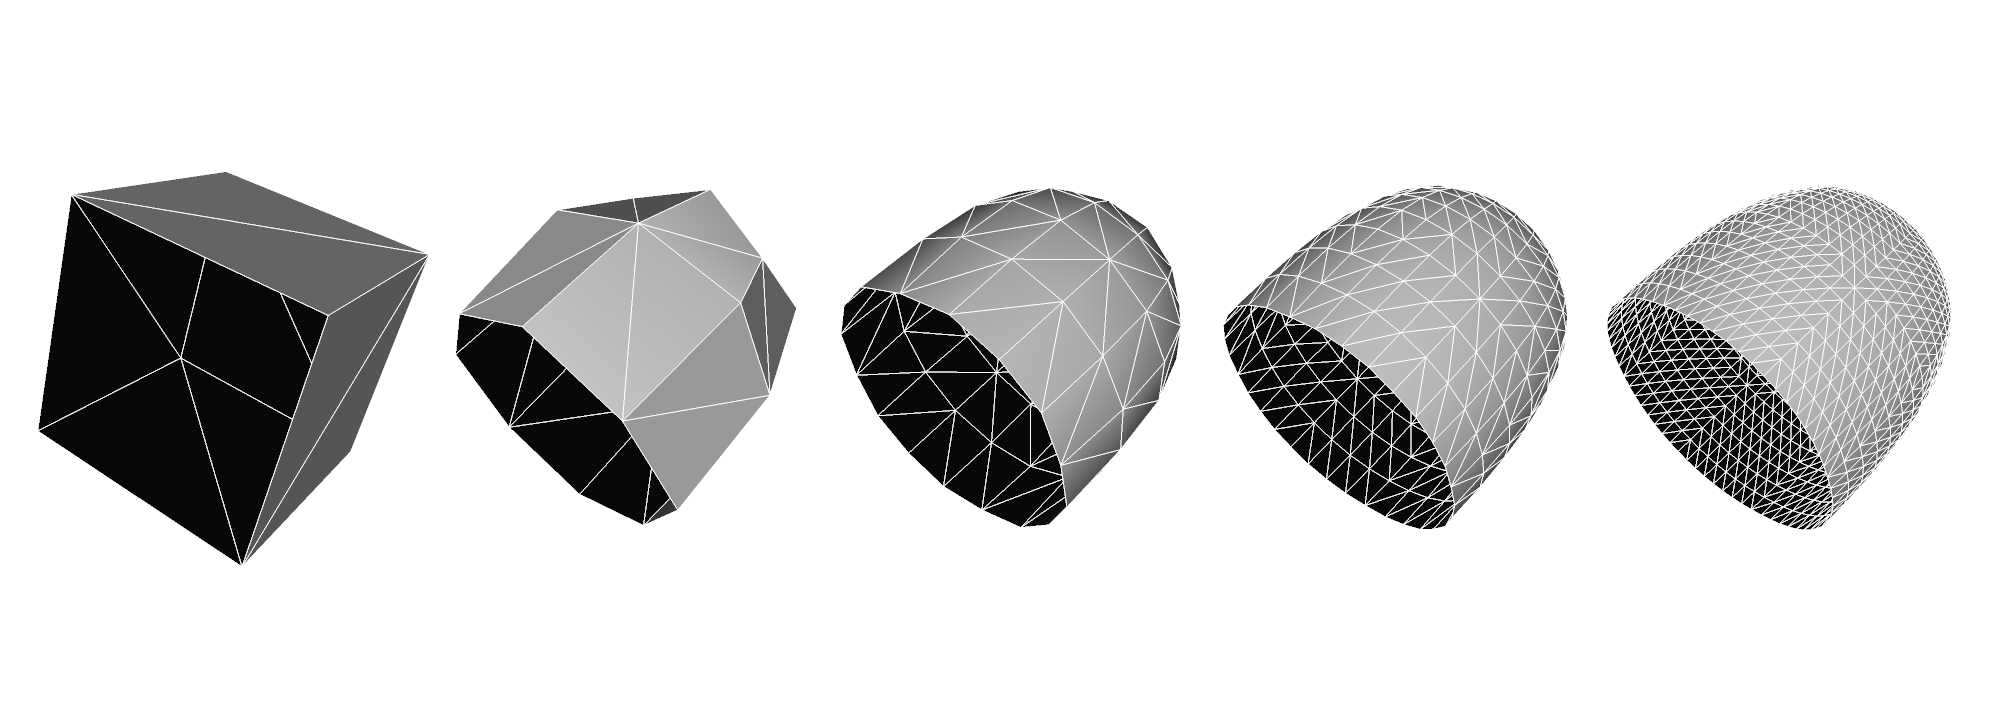
\includegraphics[scale=1.0]{cube_holes.png}
    \caption{Пять итераций сглаживания модели куба без одной грани}
\end{figure}

% Здесь уже ничего не добавится, скорее всего, переносим подзаголовок
\newpage
\subsection{Производительность}
Производительность оценивалась в двух основных сценариях: 
\begin{enumerate}
    \item На небольших сетках (около 30,000 вершин), на которых необходимо было достичь такого уровня производительности, чтобы две итерации сглаживания происходили не более чем за 16 мсек, вписываясь таким образом во временной бюджет приложения, работающего в реальном времени.
    \item На больших сетках (более 10,000,000 вершин), на которых время работы достаточно для оценки масштабируемости параллельной версии программы.
\end{enumerate}

Все оценки были получены усреднением времени, полученного на 25 повторных запусках программы. При запусках программы на больших сетках среднеквадратическое отклонение времени работы не превышало 2\%.

На небольших сетках в итоге удалось только приблизиться к необходимому уровню производительности: сетки из 30,000 вершин программа сглаживает на две итерации за 20 мсек. Таким образом реализация применима для работы в режиме 30 кадров в секунду, но не 60.

% На больших сетках получены следующие результаты: сетка из 13,000,000 вершин (прибл. 800МБ) сглаживается за 1.85 секунд, сетка из 31,000,000 вершин (прибл. 1.5ГБ) сглаживается за 3.77 секунд.

Для оценки времени работы в зависимости от размера сетки был построен график, по которому можно заключить, что программа обладает линейной ассимптотической сложностью:

\begin{figure}[H]
    \centering
    
    \begin{tikzpicture}
	\begin{loglogaxis}[xlabel={Вершины}, ylabel={Время, мс}]
   	    \addplot[color=black,mark=x] coordinates {
            (124212, 10)
            (494440, 35.9)
            (1972188, 200)
            (7877740, 853)
            (31485336, 3060.9)
      	};
	    \end{loglogaxis}
    \end{tikzpicture}
    \caption{Зависимость времени работы программы от размера сетки}
\end{figure}

\subsection{Масштабируемость}
Для оценки масштабируемости программа запускалась на 6-ядерном процессоре \texttt{AMD Ryzen 1600} на сетке размером приблизительно 7.8 млн вершин. Для оценки производительности при одном потоке использовалась последовательная версия программы.
\begin{figure}[H]
    \centering
    \begin{subfigure}{0.45\textwidth}
    \begin{tikzpicture}
        \begin{axis}[xlabel={Количество потоков}, y tick label style={rotate=45}]
   	    \addplot[color=black,mark=x] coordinates {
            (1, 1251.7)
            (2, 954.4)
            (3, 813.9)
            (4, 748.1)
            (5, 728.3)
            (6, 733.3)
      	};
	    \end{axis}
    \end{tikzpicture}
    \end{subfigure}
    \begin{subfigure}{0.45\textwidth}
    \begin{tikzpicture}
        \begin{axis}[xlabel={Количество потоков}, y tick label style={rotate=45}]
   	    \addplot[color=black,mark=x] coordinates {
            (1, 1)
            (2, 1251.7 / 954.4)
            (3, 1251.7 / 813.9)
            (4, 1251.7 / 748.1)
            (5, 1251.7 / 728.3)
            (6, 1251.7 / 733.3)
      	};
	    \end{axis}
    \end{tikzpicture}
    \end{subfigure}
    \caption{Графики времени работы в мс (a) и ускорения (b) от количества потоков}
\end{figure}

Как можно заметить, полученное ускорение далеко от теоретического максимума: эффективность параллельной программы на 6 потоках равна приблизительно 0.28. Окончательного решения этой проблемы найти не удалось, однако были предприняты следующие действия:
\begin{enumerate}
    \item Произведено сравнение времен работы отдельных сегментов программы в последовательной и параллельной версии, с тем чтобы обнаружить какие именно сегменты плохо масштабируются. Практически все сегменты программы показали на 6 потоках ускорение близкое к 3. Однако два этапа: расчет точек граней и построение граней сглаженной сетки ускорились в 2.06 и 1.3 раза, соответственно.
        \begin{figure}[H]
            \centering
        \begin{tabular}{|l | c | c | c |}
            Этап & Время 1П & Время 6П & Ускорение \\
            \hline
            Подсчет всех ребер & 20.5 & 7.8 & 2.63 \\
            Подсчет уникальных ребер & 86.7 & 31.7 & 2.74 \\
            \textbf{Расчет точек граней} & \textbf{6.8} & \textbf{3.3} & \textbf{2.06} \\
            Расчет точек ребер & 61.2 & 25.1 & 2.44 \\
            Пересчет координат & 35.2 & 12.9 & 2.73 \\
            \textbf{Построение граней} & \textbf{13.5} & \textbf{10.4} & \textbf{1.3} \\
    \end{tabular}
            \captionof{table}{Сравнение времени работы отдельных этапов программы на одном и шести потоках}
        \end{figure}
    \item Этап построения граней был выделен в отдельную программу для более детального изучения. После сравнения количества данных, записываемых в память и пропускной способности памяти был сделан вывод, что этот этап программы ограничен пропускной способностью памяти (memory bound). Действительно, этот этап программы по сути не содержит никаких расчетов, а на каждой итерации цикла считывается $(2N + 1) \cdot 4$ байт и записывается $16 \cdot N$ байт, где $N$ ---
        количество вершин в грани. Аналогичная проблема, хоть и в меньшей степени, мешает масштабированию расчета точек граней: на каждые 4 считанные из памяти байта приходится всего одна операция сложения, а на каждые $4 \cdot N$ байт --- одна операция умножения.
    \item Выбранный способ распараллеливания на этапах подсчета уникальных ребер и расчета точек ребер тем менее эффективен, чем больше потоков выделено для решения задачи. В случае подсчета уникальных ребер, количество потоков прямо пропорционально количеству итераций, на которых поток не будет делать никакой работы. Оба названных этапа страдают от неравномерной нагруженности потоков, так как между потоками распределяются не ребра, а вершины. В отдельной ветви разработки
        была протестирована версия программы, в которой за счет более сложной схемы разделения работы каждому потоку выделяется равное количество ребер, а не вершин, однако, время, затраченное на вычисление количества работы, оказалось больше полученного выигрыша. Таким образом, проблема неравномерной нагруженности потоков на этих этапах осталась нерешенной.
\end{enumerate}

\newpage
\section{Заключение}
В ходе выполнения курсовой работы был изучен алгоритм Кэтмелла-Кларка и реализована последовательная и параллельная версия программы. Была проведена работа по оптимизации, в ходе которой не удалось достигнуть уровня, сравнимого с реализацией OpenSubdiv, однако полученная реализация позволяет производить манипуляции с сетками размером до 30,000 вершин в режиме 30 кадров в секунду. Была изучена масштабируемость параллельной версии программы и найдены сегменты, масштабируемость которых
ограничивается пропускной способностью памяти.

Дальнейшая работа может быть сосредоточена на:
\begin{enumerate}
\item Реализации алгоритма для систем с распределенной памятью
\item Дальнейших алгоритмических и программных оптимизациях
\item Изучении возможности сжатия данных для уменьшения воздействия пропускной способности памяти на быстродействие алгоритма.
\end{enumerate}

\newpage
\addcontentsline{toc}{section}{Список литературы}
\begin{thebibliography}{9}
\bibitem{rogers01} Р. Роджерс, Дж. Адамс. \textit{Математитечские основы машинной графики}, Москва, 2001
\bibitem{catmark79}
    E. Catnull, J. Clark. \textit{Recursively generated B-spline surfaces on arbitrary topological meshes}. Computer-Aided Design 10 (6), 1978
\bibitem{opensubdivWWW} Why Fast Subdivision? \textit{Pixar OpenSubdiv}. Электронный ресурс. Режим доступа: \url{http://graphics.pixar.com/opensubdiv/docs/intro.html} (дата обращения 10.06.2020)
\bibitem{objWWW} Wavefront OBJ File Format. \textit{Digital Preservation at the Library of Congress}. Электронный ресурс. Режим доступа: \url{https://www.loc.gov/preservation/digital/formats/fdd/fdd000507.shtml} (дата обращения 10.06.2020)
\bibitem{voevodin02} В.В.Воеводин, Вл.В.Воеводин. \textit{Параллельные вычисления}, БХВ-Петербург, 2002
\bibitem{kasper03} К. Касперски. \textit{Техника оптимизации программ. Эффективное использование памяти}, БХВ-Петербург, 2001
\end{thebibliography}

\end{document}
